\documentclass{beamer}
\author{Shadrach Kwakye-Nimo}
\title{Evaluation of the relaxation of plastic melt}
\begin{document}

\begin{frame}
\titlepage
\end{frame}


\begin{frame}
The relaxation of a plastic melt was evaluated by solving a modified version of the diffusion equation. The program is able to estimate the amount of stress relaxation in the plastic melt at any given time. 
\end{frame}

\begin{frame}
For the HDPE used in this simulation, the stress relaxation modulus is shown below.
\begin{figure}
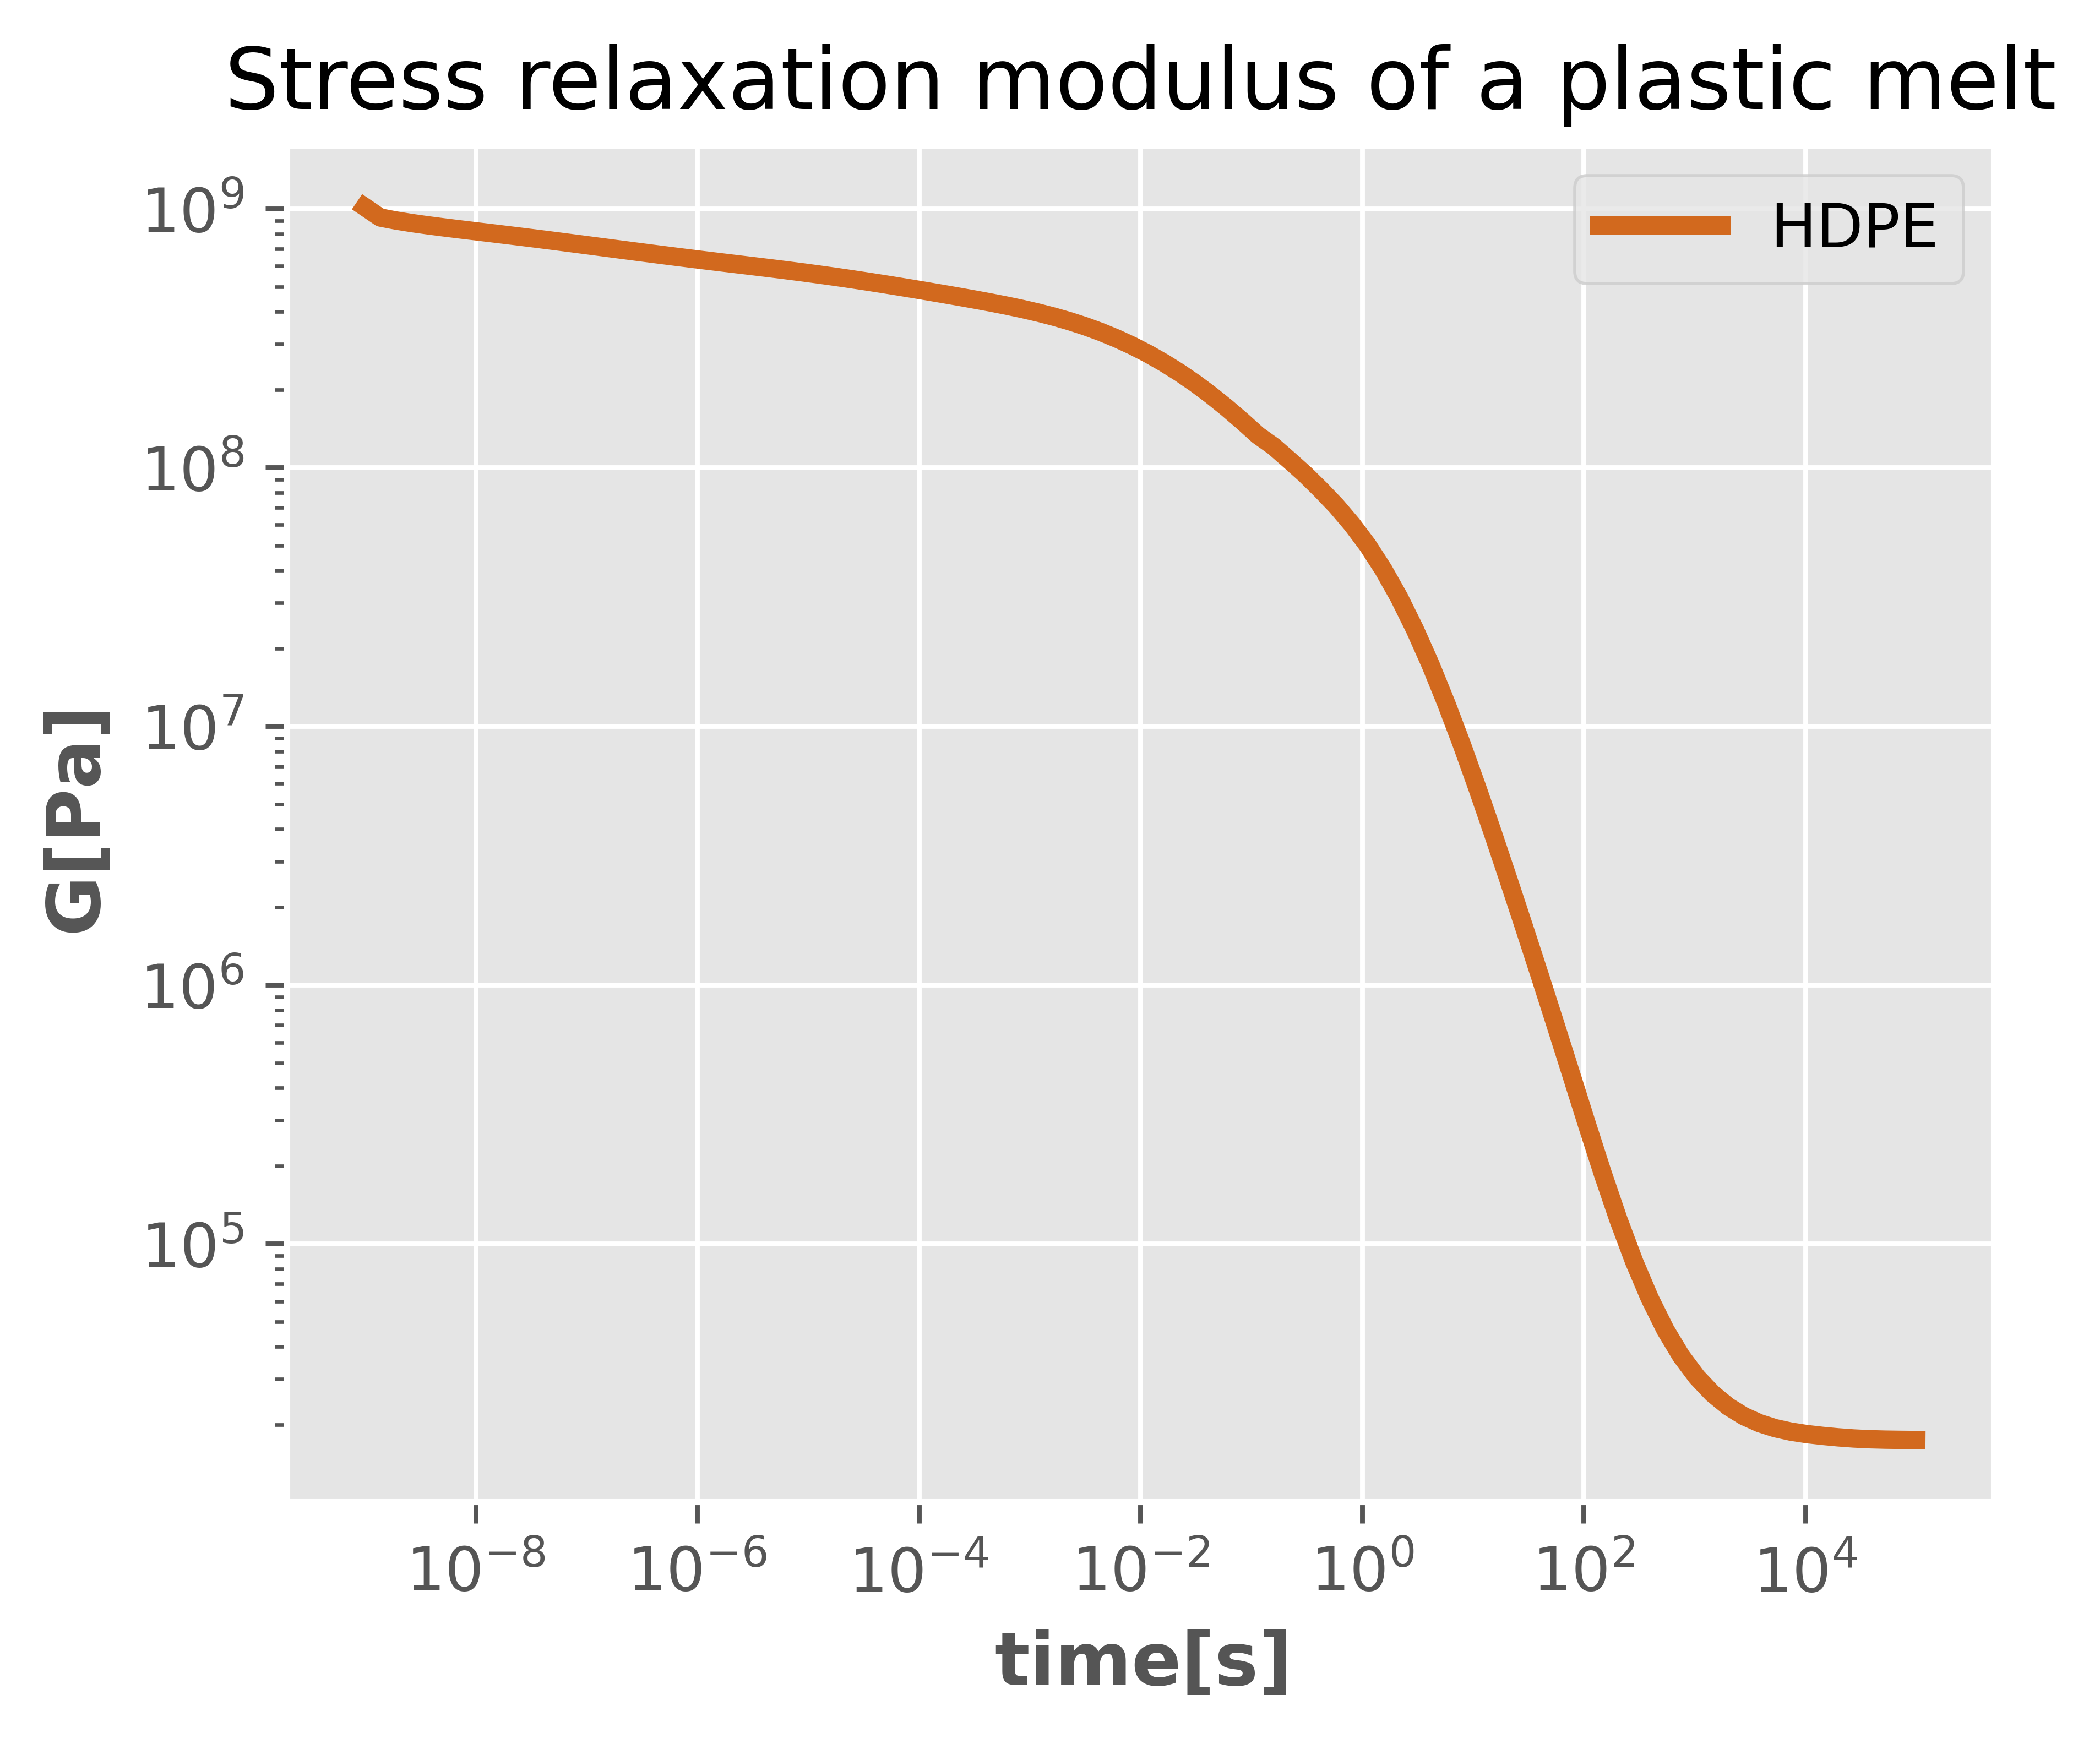
\includegraphics[scale=0.7]{figures/relaxation.png}
\end{figure}

\end{frame}


\begin{frame}
\frametitle{contour lenght fluctuations}
Observing the contour length fluctuation over half the chain's length for a chain of weight $297831 g/mol$ and comparing it to \textit{Pattamaprom et al.(2000)} as a means of validation.

\begin{figure}
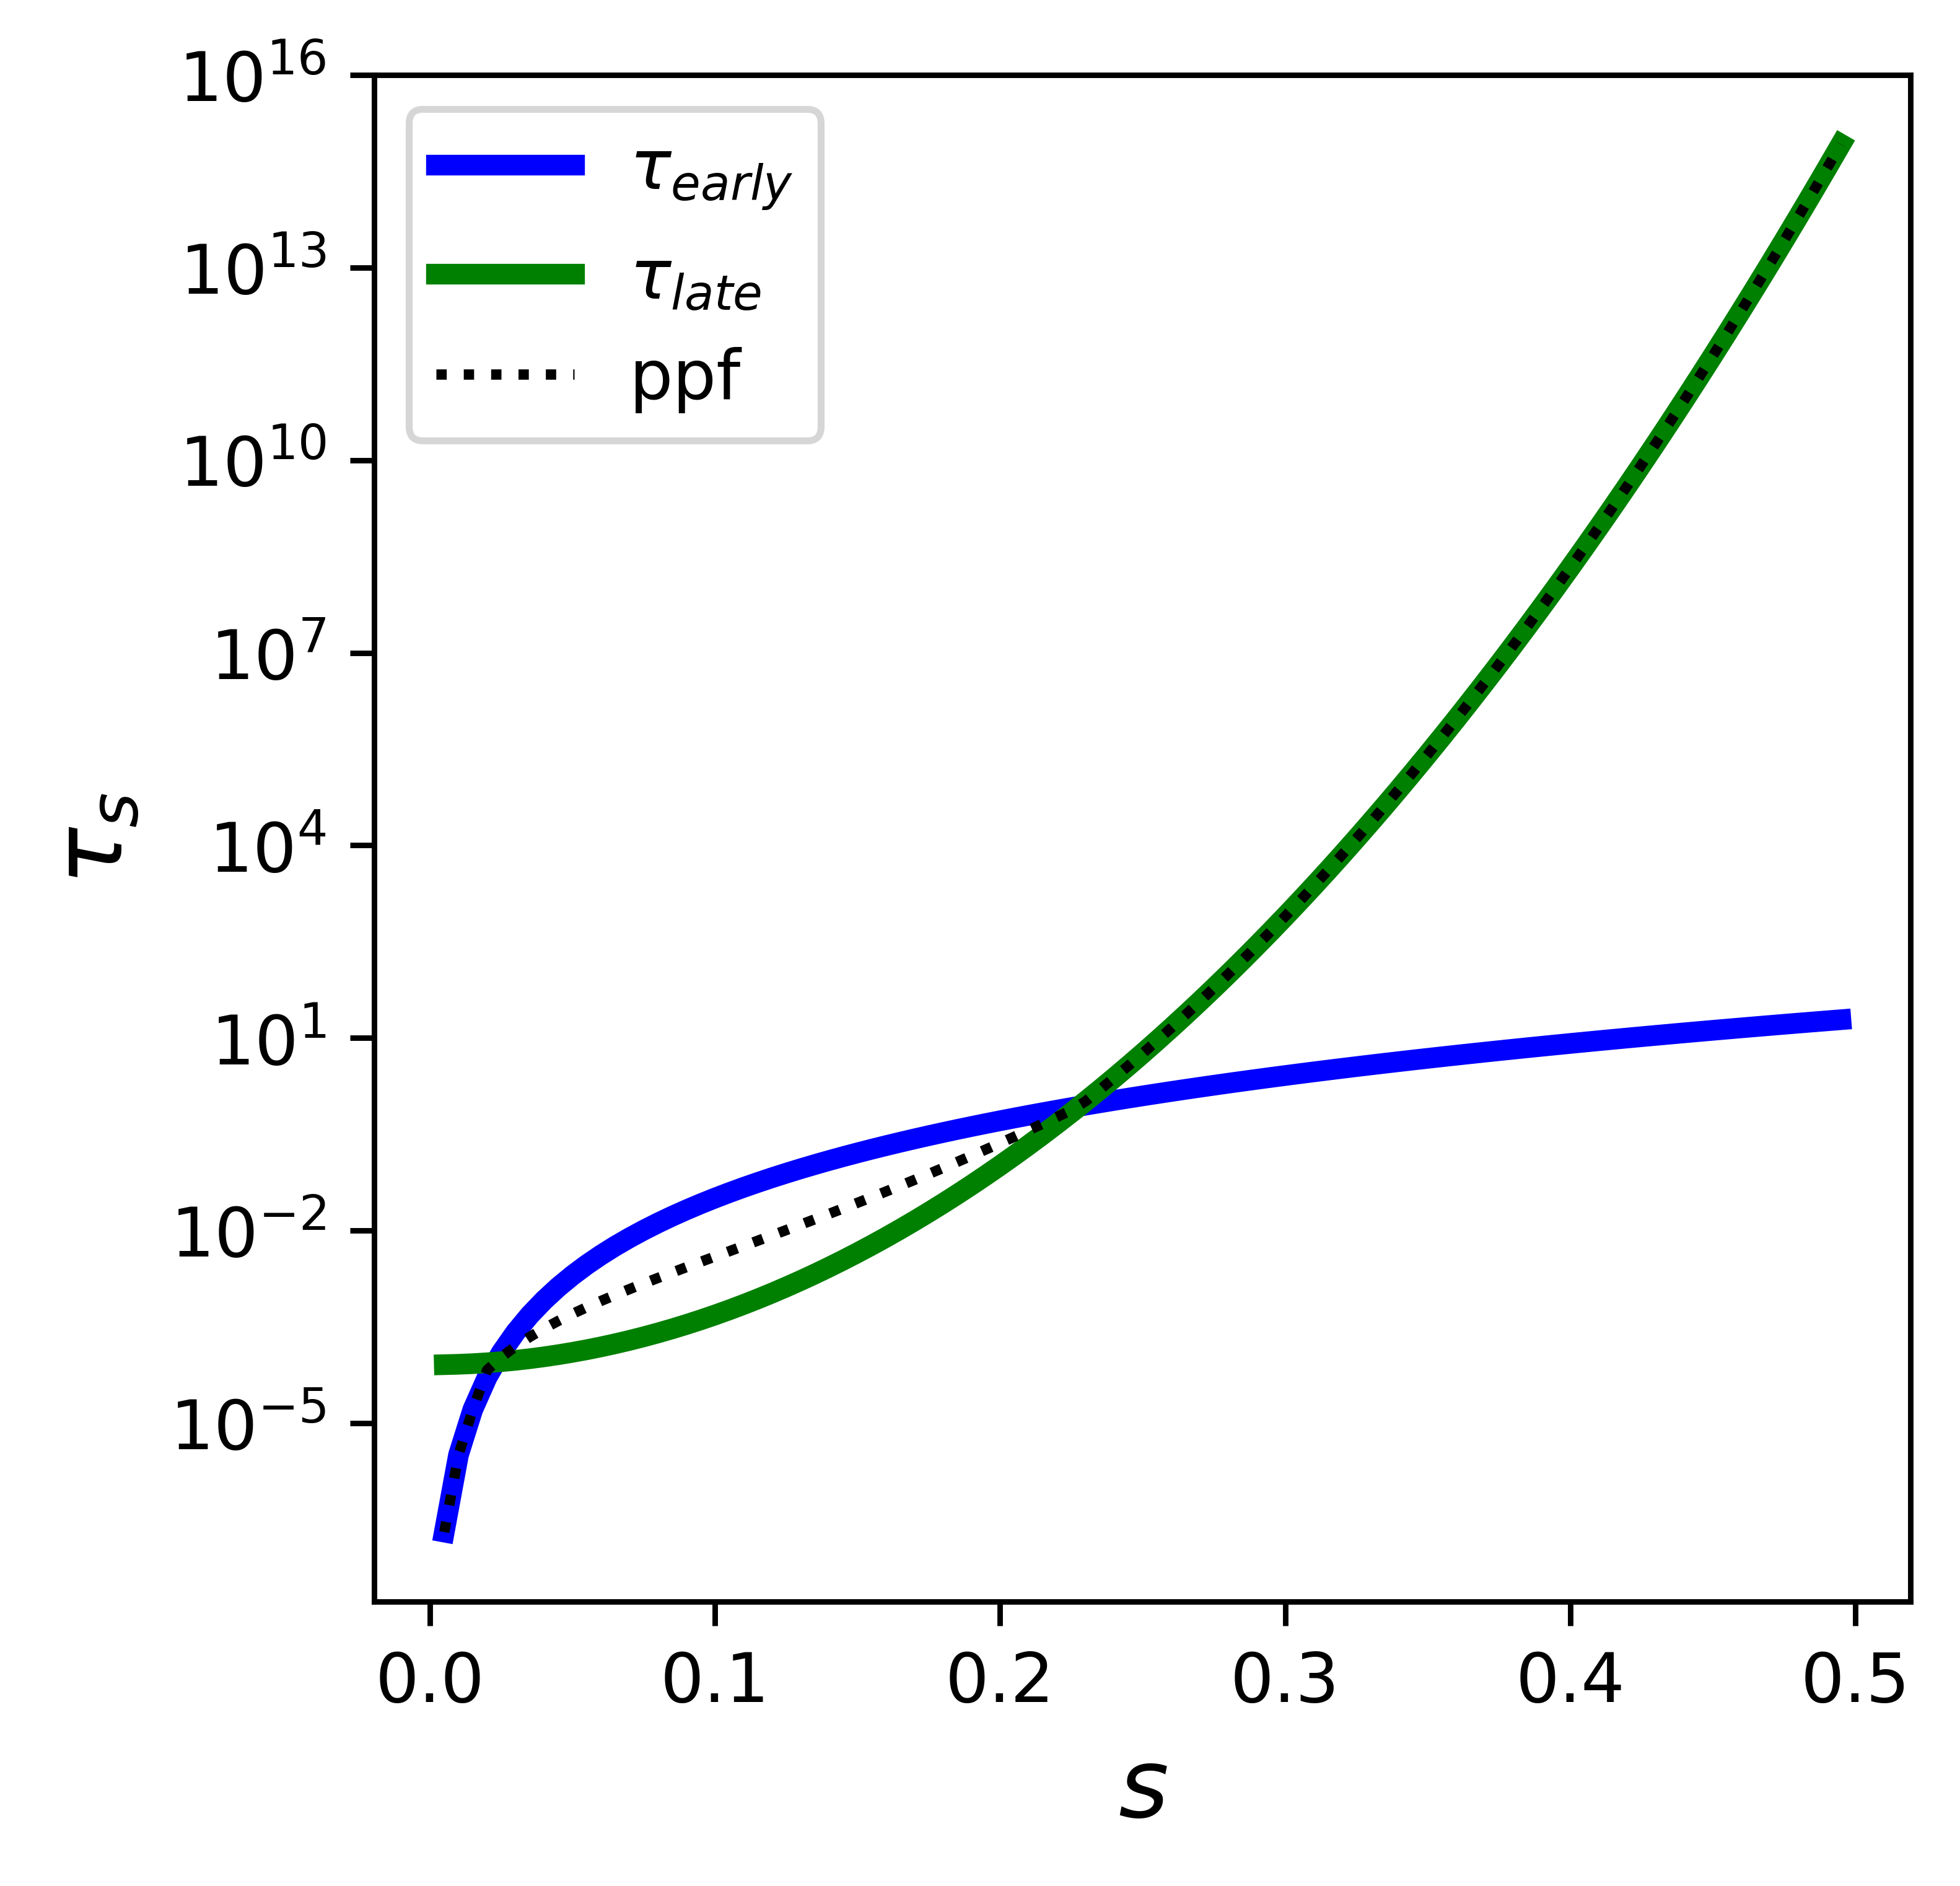
\includegraphics[scale=0.7]{figures/ppf.png}
\end{figure}

\end{frame}



\begin{frame}
\frametitle{reference}
\begin{thebibliography}{10}
\bibitem{Pattamaprom2000}
\alert{Pattamaprom, C., Larson, R. G., \& Van Dyke, T. J.}
\newblock  {Quantitative predictions of linear viscoelastic rheological properties of entangled polymers.}
\newblock {\em Rheologica Acta 39 (2000): 517-531.}.

\bibitem{Kwakye-Nimo2022}
\alert{Shadrach Kwakye-Nimo, Yongwoo Inn, Youlu Yu, and Paula M. Wood-Adams}
\newblock {Polymer Fractionation at an Interface in Simple Shear with Slip}
\newblock {\em Macromolecules 55.15 (2022): 6609-6619.}.
\end{thebibliography}

\end{frame}

\end{document}